% Options for packages loaded elsewhere
\PassOptionsToPackage{unicode}{hyperref}
\PassOptionsToPackage{hyphens}{url}
%
\documentclass[
]{article}
\usepackage{amsmath,amssymb}
\usepackage{iftex}
\ifPDFTeX
  \usepackage[T1]{fontenc}
  \usepackage[utf8]{inputenc}
  \usepackage{textcomp} % provide euro and other symbols
\else % if luatex or xetex
  \usepackage{unicode-math} % this also loads fontspec
  \defaultfontfeatures{Scale=MatchLowercase}
  \defaultfontfeatures[\rmfamily]{Ligatures=TeX,Scale=1}
\fi
\usepackage{lmodern}
\ifPDFTeX\else
  % xetex/luatex font selection
\fi
% Use upquote if available, for straight quotes in verbatim environments
\IfFileExists{upquote.sty}{\usepackage{upquote}}{}
\IfFileExists{microtype.sty}{% use microtype if available
  \usepackage[]{microtype}
  \UseMicrotypeSet[protrusion]{basicmath} % disable protrusion for tt fonts
}{}
\makeatletter
\@ifundefined{KOMAClassName}{% if non-KOMA class
  \IfFileExists{parskip.sty}{%
    \usepackage{parskip}
  }{% else
    \setlength{\parindent}{0pt}
    \setlength{\parskip}{6pt plus 2pt minus 1pt}}
}{% if KOMA class
  \KOMAoptions{parskip=half}}
\makeatother
\usepackage{xcolor}
\usepackage[margin=1in]{geometry}
\usepackage{color}
\usepackage{fancyvrb}
\newcommand{\VerbBar}{|}
\newcommand{\VERB}{\Verb[commandchars=\\\{\}]}
\DefineVerbatimEnvironment{Highlighting}{Verbatim}{commandchars=\\\{\}}
% Add ',fontsize=\small' for more characters per line
\usepackage{framed}
\definecolor{shadecolor}{RGB}{248,248,248}
\newenvironment{Shaded}{\begin{snugshade}}{\end{snugshade}}
\newcommand{\AlertTok}[1]{\textcolor[rgb]{0.94,0.16,0.16}{#1}}
\newcommand{\AnnotationTok}[1]{\textcolor[rgb]{0.56,0.35,0.01}{\textbf{\textit{#1}}}}
\newcommand{\AttributeTok}[1]{\textcolor[rgb]{0.13,0.29,0.53}{#1}}
\newcommand{\BaseNTok}[1]{\textcolor[rgb]{0.00,0.00,0.81}{#1}}
\newcommand{\BuiltInTok}[1]{#1}
\newcommand{\CharTok}[1]{\textcolor[rgb]{0.31,0.60,0.02}{#1}}
\newcommand{\CommentTok}[1]{\textcolor[rgb]{0.56,0.35,0.01}{\textit{#1}}}
\newcommand{\CommentVarTok}[1]{\textcolor[rgb]{0.56,0.35,0.01}{\textbf{\textit{#1}}}}
\newcommand{\ConstantTok}[1]{\textcolor[rgb]{0.56,0.35,0.01}{#1}}
\newcommand{\ControlFlowTok}[1]{\textcolor[rgb]{0.13,0.29,0.53}{\textbf{#1}}}
\newcommand{\DataTypeTok}[1]{\textcolor[rgb]{0.13,0.29,0.53}{#1}}
\newcommand{\DecValTok}[1]{\textcolor[rgb]{0.00,0.00,0.81}{#1}}
\newcommand{\DocumentationTok}[1]{\textcolor[rgb]{0.56,0.35,0.01}{\textbf{\textit{#1}}}}
\newcommand{\ErrorTok}[1]{\textcolor[rgb]{0.64,0.00,0.00}{\textbf{#1}}}
\newcommand{\ExtensionTok}[1]{#1}
\newcommand{\FloatTok}[1]{\textcolor[rgb]{0.00,0.00,0.81}{#1}}
\newcommand{\FunctionTok}[1]{\textcolor[rgb]{0.13,0.29,0.53}{\textbf{#1}}}
\newcommand{\ImportTok}[1]{#1}
\newcommand{\InformationTok}[1]{\textcolor[rgb]{0.56,0.35,0.01}{\textbf{\textit{#1}}}}
\newcommand{\KeywordTok}[1]{\textcolor[rgb]{0.13,0.29,0.53}{\textbf{#1}}}
\newcommand{\NormalTok}[1]{#1}
\newcommand{\OperatorTok}[1]{\textcolor[rgb]{0.81,0.36,0.00}{\textbf{#1}}}
\newcommand{\OtherTok}[1]{\textcolor[rgb]{0.56,0.35,0.01}{#1}}
\newcommand{\PreprocessorTok}[1]{\textcolor[rgb]{0.56,0.35,0.01}{\textit{#1}}}
\newcommand{\RegionMarkerTok}[1]{#1}
\newcommand{\SpecialCharTok}[1]{\textcolor[rgb]{0.81,0.36,0.00}{\textbf{#1}}}
\newcommand{\SpecialStringTok}[1]{\textcolor[rgb]{0.31,0.60,0.02}{#1}}
\newcommand{\StringTok}[1]{\textcolor[rgb]{0.31,0.60,0.02}{#1}}
\newcommand{\VariableTok}[1]{\textcolor[rgb]{0.00,0.00,0.00}{#1}}
\newcommand{\VerbatimStringTok}[1]{\textcolor[rgb]{0.31,0.60,0.02}{#1}}
\newcommand{\WarningTok}[1]{\textcolor[rgb]{0.56,0.35,0.01}{\textbf{\textit{#1}}}}
\usepackage{graphicx}
\makeatletter
\def\maxwidth{\ifdim\Gin@nat@width>\linewidth\linewidth\else\Gin@nat@width\fi}
\def\maxheight{\ifdim\Gin@nat@height>\textheight\textheight\else\Gin@nat@height\fi}
\makeatother
% Scale images if necessary, so that they will not overflow the page
% margins by default, and it is still possible to overwrite the defaults
% using explicit options in \includegraphics[width, height, ...]{}
\setkeys{Gin}{width=\maxwidth,height=\maxheight,keepaspectratio}
% Set default figure placement to htbp
\makeatletter
\def\fps@figure{htbp}
\makeatother
\setlength{\emergencystretch}{3em} % prevent overfull lines
\providecommand{\tightlist}{%
  \setlength{\itemsep}{0pt}\setlength{\parskip}{0pt}}
\setcounter{secnumdepth}{-\maxdimen} % remove section numbering
\usepackage{booktabs}
\usepackage{caption}
\usepackage{longtable}
\usepackage{colortbl}
\usepackage{array}
\usepackage{anyfontsize}
\usepackage{multirow}
\ifLuaTeX
  \usepackage{selnolig}  % disable illegal ligatures
\fi
\usepackage{bookmark}
\IfFileExists{xurl.sty}{\usepackage{xurl}}{} % add URL line breaks if available
\urlstyle{same}
\hypersetup{
  pdftitle={Lab Assignment 7},
  pdfauthor={Summer Heschong},
  hidelinks,
  pdfcreator={LaTeX via pandoc}}

\title{Lab Assignment 7}
\author{Summer Heschong}
\date{2025-02-26}

\begin{document}
\maketitle

\#Setup

\begin{Shaded}
\begin{Highlighting}[]
\FunctionTok{library}\NormalTok{(here)}
\end{Highlighting}
\end{Shaded}

\begin{verbatim}
## here() starts at /Users/summerheschong/stats_spring25
\end{verbatim}

\begin{Shaded}
\begin{Highlighting}[]
\FunctionTok{library}\NormalTok{(tidyverse)}
\end{Highlighting}
\end{Shaded}

\begin{verbatim}
## -- Attaching core tidyverse packages ------------------------ tidyverse 2.0.0 --
## v dplyr     1.1.4     v readr     2.1.5
## v forcats   1.0.0     v stringr   1.5.1
## v ggplot2   3.5.1     v tibble    3.2.1
## v lubridate 1.9.4     v tidyr     1.3.1
## v purrr     1.0.2
\end{verbatim}

\begin{verbatim}
## -- Conflicts ------------------------------------------ tidyverse_conflicts() --
## x dplyr::filter() masks stats::filter()
## x dplyr::lag()    masks stats::lag()
## i Use the conflicted package (<http://conflicted.r-lib.org/>) to force all conflicts to become errors
\end{verbatim}

\begin{Shaded}
\begin{Highlighting}[]
\FunctionTok{library}\NormalTok{(dunn.test)}
\FunctionTok{library}\NormalTok{(gt)}
\FunctionTok{library}\NormalTok{(paletteer)}

\CommentTok{\#load data set}
\NormalTok{vert\_data }\OtherTok{\textless{}{-}} \FunctionTok{read.csv}\NormalTok{(}\FunctionTok{here}\NormalTok{(}\StringTok{\textquotesingle{}Data/Raw/and\_vertebrates.csv\textquotesingle{}}\NormalTok{))}

\CommentTok{\#filter data set for cutthroat trout}
\NormalTok{trout\_data }\OtherTok{\textless{}{-}}\NormalTok{ vert\_data }\SpecialCharTok{\%\textgreater{}\%}
  \FunctionTok{filter}\NormalTok{(species }\SpecialCharTok{==} \StringTok{\textquotesingle{}Cutthroat trout\textquotesingle{}}\NormalTok{)}
\end{Highlighting}
\end{Shaded}

\#(1) Mann-Whitney U and Wilcoxon Signed-Rank Tests \#\#a. Examine
normality of data and run a Mann-Whitney U test

\begin{Shaded}
\begin{Highlighting}[]
\CommentTok{\#visualize data}
\NormalTok{fig1 }\OtherTok{\textless{}{-}} \FunctionTok{ggplot}\NormalTok{(trout\_data, }\FunctionTok{aes}\NormalTok{(}\AttributeTok{x =}\NormalTok{ length\_1\_mm, }\AttributeTok{fill =}\NormalTok{ section)) }\SpecialCharTok{+}
  \FunctionTok{geom\_histogram}\NormalTok{(}\AttributeTok{bins =} \DecValTok{30}\NormalTok{, }\AttributeTok{binwidth =} \DecValTok{6}\NormalTok{, }\AttributeTok{color =} \StringTok{\textquotesingle{}black\textquotesingle{}}\NormalTok{) }\SpecialCharTok{+}
  \FunctionTok{facet\_wrap}\NormalTok{(}\SpecialCharTok{\textasciitilde{}}\NormalTok{section) }\SpecialCharTok{+}
  \FunctionTok{labs}\NormalTok{(}\AttributeTok{title =} \StringTok{\textquotesingle{}Cutthroat Trout Length by Forest Treatment\textquotesingle{}}\NormalTok{, }
       \AttributeTok{x =} \StringTok{\textquotesingle{}snout{-}to{-}fork length (mm)\textquotesingle{}}\NormalTok{)}
\NormalTok{fig1}
\end{Highlighting}
\end{Shaded}

\begin{verbatim}
## Warning: Removed 5 rows containing non-finite outside the scale range
## (`stat_bin()`).
\end{verbatim}

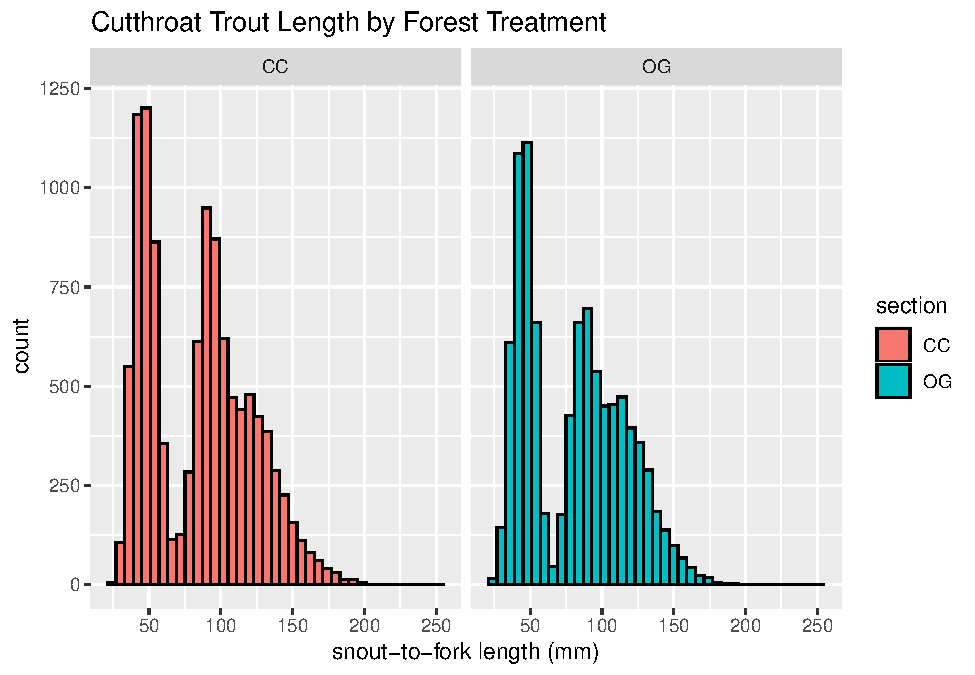
\includegraphics{Lab7_Summer.Heschong_files/figure-latex/MannWhitney U Test-1.pdf}

\begin{Shaded}
\begin{Highlighting}[]
\CommentTok{\#run Mann{-}Whitney U test}

\CommentTok{\#First separate fish lengths by forest treatment type}
\NormalTok{CCtrout\_data }\OtherTok{\textless{}{-}}\NormalTok{ trout\_data }\SpecialCharTok{\%\textgreater{}\%}
  \FunctionTok{filter}\NormalTok{(section }\SpecialCharTok{==} \StringTok{\textquotesingle{}CC\textquotesingle{}}\NormalTok{)}
\NormalTok{OGtrout\_data }\OtherTok{\textless{}{-}}\NormalTok{ trout\_data }\SpecialCharTok{\%\textgreater{}\%}
  \FunctionTok{filter}\NormalTok{(section }\SpecialCharTok{==} \StringTok{\textquotesingle{}OG\textquotesingle{}}\NormalTok{)}

\CommentTok{\#Are ranks of fish lengths significantly different between forest treatment types?}
\FunctionTok{wilcox.test}\NormalTok{(CCtrout\_data}\SpecialCharTok{$}\NormalTok{length\_1\_mm, }
\NormalTok{            OGtrout\_data}\SpecialCharTok{$}\NormalTok{length\_1\_mm, }
            \AttributeTok{paired =} \ConstantTok{FALSE}\NormalTok{)}
\end{Highlighting}
\end{Shaded}

\begin{verbatim}
## 
##  Wilcoxon rank sum test with continuity correction
## 
## data:  CCtrout_data$length_1_mm and OGtrout_data$length_1_mm
## W = 55178843, p-value = 7.697e-16
## alternative hypothesis: true location shift is not equal to 0
\end{verbatim}

Answer: There was a significant difference in ranks between cutthroat
trout snout-to-fork length in clear-cut forest (median = 88mm, IQR =
50-111mm) and in old growth forests (median = 84mm, IQR = 48-108mm) as
determined by a Mann-Whitney U Test (W = 55,178,843, p = 7.7e-16).

\#\#b. Visualize data to assess normality and run a Wilcoxon Signed-Rank
test

\begin{Shaded}
\begin{Highlighting}[]
\CommentTok{\#load in new dataset}
\NormalTok{recapture\_data }\OtherTok{\textless{}{-}} \FunctionTok{read.csv}\NormalTok{(}\FunctionTok{here}\NormalTok{(}\StringTok{\textquotesingle{}Data/Raw/trout\_recapture\_v2.csv\textquotesingle{}}\NormalTok{))}

\CommentTok{\#visualize data}
\NormalTok{fig2 }\OtherTok{\textless{}{-}} \FunctionTok{ggplot}\NormalTok{(recapture\_data, }\FunctionTok{aes}\NormalTok{(}\AttributeTok{x =}\NormalTok{ length\_1\_mm, }\AttributeTok{fill =}\NormalTok{ year)) }\SpecialCharTok{+}
  \FunctionTok{geom\_histogram}\NormalTok{(}\AttributeTok{bins =} \DecValTok{11}\NormalTok{, }\AttributeTok{binwidth =} \DecValTok{7}\NormalTok{, }\AttributeTok{color =} \StringTok{\textquotesingle{}black\textquotesingle{}}\NormalTok{) }\SpecialCharTok{+}
  \FunctionTok{facet\_wrap}\NormalTok{(}\SpecialCharTok{\textasciitilde{}}\NormalTok{year) }\SpecialCharTok{+}
  \FunctionTok{labs}\NormalTok{(}\AttributeTok{title =} \StringTok{\textquotesingle{}Cutthroat Trout Length by Year\textquotesingle{}}\NormalTok{, }
       \AttributeTok{x =} \StringTok{\textquotesingle{}snout{-}to{-}fork length (mm)\textquotesingle{}}\NormalTok{)}
\NormalTok{fig2}
\end{Highlighting}
\end{Shaded}

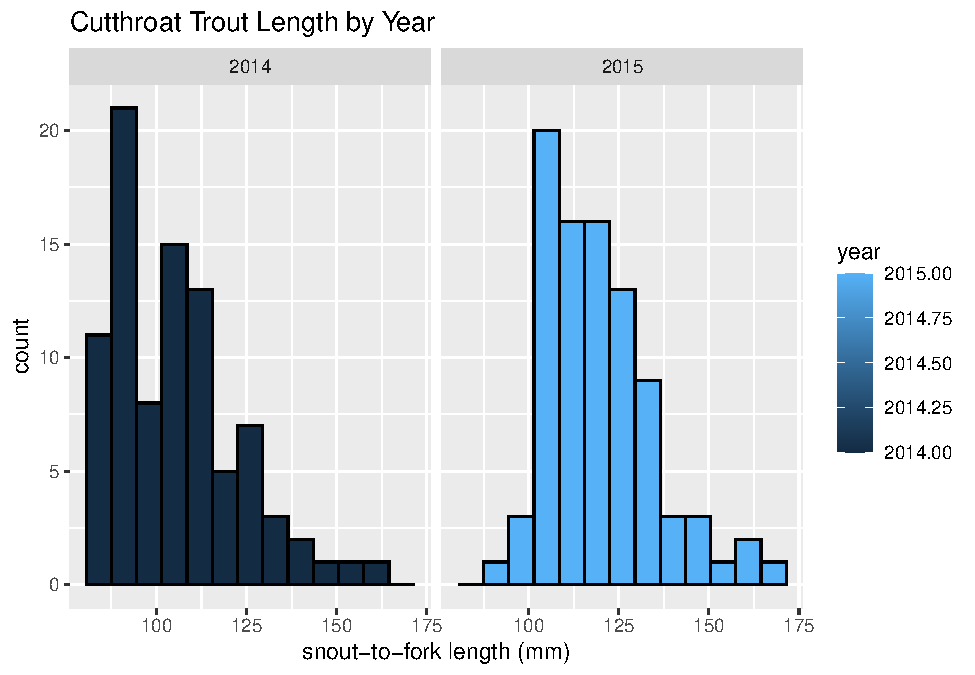
\includegraphics{Lab7_Summer.Heschong_files/figure-latex/Wilcoxon Signed-Rank test-1.pdf}

\begin{Shaded}
\begin{Highlighting}[]
\CommentTok{\#run Wilcoxon Signed{-}Rank test}
\CommentTok{\#first separate data by year}
\NormalTok{trout2014 }\OtherTok{\textless{}{-}}\NormalTok{ recapture\_data }\SpecialCharTok{\%\textgreater{}\%}
  \FunctionTok{filter}\NormalTok{(year }\SpecialCharTok{==} \StringTok{\textquotesingle{}2014\textquotesingle{}}\NormalTok{)}
\NormalTok{trout2015 }\OtherTok{\textless{}{-}}\NormalTok{ recapture\_data }\SpecialCharTok{\%\textgreater{}\%}
  \FunctionTok{filter}\NormalTok{(year }\SpecialCharTok{==} \StringTok{\textquotesingle{}2015\textquotesingle{}}\NormalTok{)}

\CommentTok{\#Are ranks of fish lengths significantly different between years?}
\FunctionTok{wilcox.test}\NormalTok{(trout2014}\SpecialCharTok{$}\NormalTok{length\_1\_mm, }
\NormalTok{            trout2015}\SpecialCharTok{$}\NormalTok{length\_1\_mm, }
            \AttributeTok{paired =} \ConstantTok{TRUE}\NormalTok{)}
\end{Highlighting}
\end{Shaded}

\begin{verbatim}
## 
##  Wilcoxon signed rank test with continuity correction
## 
## data:  trout2014$length_1_mm and trout2015$length_1_mm
## V = 625.5, p-value = 4.973e-08
## alternative hypothesis: true location shift is not equal to 0
\end{verbatim}

Answer: There was a significant difference in ranks between cutthroat
trout snout-to-fork length in 2014 (median = 104mm, IQR = 91-114mm) and
in 2015 (median = 118mm, IQR = 108-127mm) as determined by a Wilcoxon
Signed Rank Test (V = 625.5, p = 4.97e-08).

\#(2) Kruskal Wallis and post-hoc Dunn's Tests \#\#a. Visualize data and
run a Kruskal Wallis test

\begin{Shaded}
\begin{Highlighting}[]
\CommentTok{\#Visualize Data}
\NormalTok{fig3 }\OtherTok{\textless{}{-}} \FunctionTok{ggplot}\NormalTok{(trout\_data, }\FunctionTok{aes}\NormalTok{(}\AttributeTok{x =}\NormalTok{ length\_1\_mm, }\AttributeTok{fill =}\NormalTok{ reach)) }\SpecialCharTok{+}
  \FunctionTok{geom\_histogram}\NormalTok{(}\AttributeTok{bins =} \DecValTok{37}\NormalTok{, }\AttributeTok{binwidth =} \DecValTok{6}\NormalTok{, }\AttributeTok{color =} \StringTok{\textquotesingle{}black\textquotesingle{}}\NormalTok{) }\SpecialCharTok{+}
  \FunctionTok{facet\_wrap}\NormalTok{(}\SpecialCharTok{\textasciitilde{}}\NormalTok{reach) }\SpecialCharTok{+}
  \FunctionTok{labs}\NormalTok{(}\AttributeTok{title =} \StringTok{\textquotesingle{}Cutthroat Trout Length by Reach\textquotesingle{}}\NormalTok{, }
       \AttributeTok{x =} \StringTok{\textquotesingle{}snout{-}to{-}fork length (mm)\textquotesingle{}}\NormalTok{)}
\NormalTok{fig3}
\end{Highlighting}
\end{Shaded}

\begin{verbatim}
## Warning: Removed 5 rows containing non-finite outside the scale range
## (`stat_bin()`).
\end{verbatim}

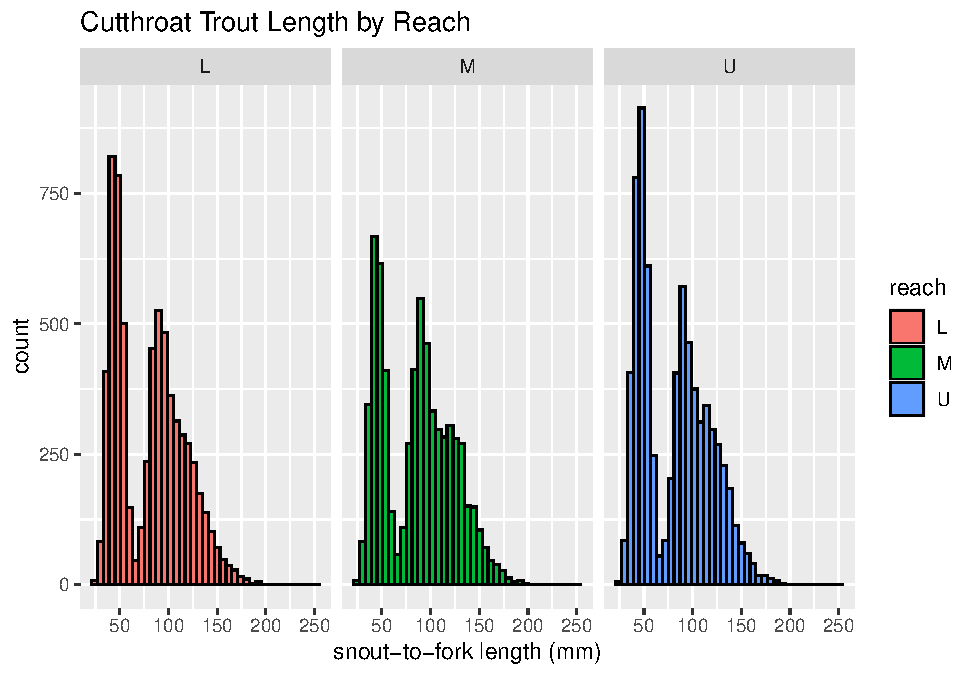
\includegraphics{Lab7_Summer.Heschong_files/figure-latex/Kruskal Wallis and Dunn Test-1.pdf}

\begin{Shaded}
\begin{Highlighting}[]
\CommentTok{\#Run a Kruskal Wallis Test to see if ranks of fish lengths are significantly different among stream reaches}
\FunctionTok{kruskal.test}\NormalTok{(length\_1\_mm }\SpecialCharTok{\textasciitilde{}}\NormalTok{ reach, }\AttributeTok{data =}\NormalTok{ trout\_data)}
\end{Highlighting}
\end{Shaded}

\begin{verbatim}
## 
##  Kruskal-Wallis rank sum test
## 
## data:  length_1_mm by reach
## Kruskal-Wallis chi-squared = 77.394, df = 2, p-value < 2.2e-16
\end{verbatim}

\begin{Shaded}
\begin{Highlighting}[]
\CommentTok{\#Ranks are significantly different {-}\textgreater{} run a Dunn\textquotesingle{}s test}
\FunctionTok{dunn.test}\NormalTok{(trout\_data}\SpecialCharTok{$}\NormalTok{length\_1\_mm, trout\_data}\SpecialCharTok{$}\NormalTok{reach)}
\end{Highlighting}
\end{Shaded}

\begin{verbatim}
##   Kruskal-Wallis rank sum test
## 
## data: x and group
## Kruskal-Wallis chi-squared = 77.3942, df = 2, p-value = 0
## 
## 
##                            Comparison of x by group                            
##                                 (No adjustment)                                
## Col Mean-|
## Row Mean |          L          M
## ---------+----------------------
##        M |  -8.305134
##          |    0.0000*
##          |
##        U |  -1.688937   6.770059
##          |     0.0456    0.0000*
## 
## alpha = 0.05
## Reject Ho if p <= alpha/2
\end{verbatim}

\begin{Shaded}
\begin{Highlighting}[]
\CommentTok{\#calculate central tendencies of reach sections for report}
\CommentTok{\#filter reach by section}
\NormalTok{reach\_L }\OtherTok{\textless{}{-}}\NormalTok{ trout\_data }\SpecialCharTok{\%\textgreater{}\%}
  \FunctionTok{filter}\NormalTok{(reach }\SpecialCharTok{==} \StringTok{\textquotesingle{}L\textquotesingle{}}\NormalTok{)}
\NormalTok{reach\_M }\OtherTok{\textless{}{-}}\NormalTok{ trout\_data }\SpecialCharTok{\%\textgreater{}\%}
  \FunctionTok{filter}\NormalTok{(reach }\SpecialCharTok{==} \StringTok{\textquotesingle{}M\textquotesingle{}}\NormalTok{)}
\NormalTok{reach\_U }\OtherTok{\textless{}{-}}\NormalTok{ trout\_data }\SpecialCharTok{\%\textgreater{}\%}
  \FunctionTok{filter}\NormalTok{(reach }\SpecialCharTok{==} \StringTok{\textquotesingle{}U\textquotesingle{}}\NormalTok{)}

\CommentTok{\#calculate medians}
\FunctionTok{median}\NormalTok{(reach\_L}\SpecialCharTok{$}\NormalTok{length\_1\_mm, }\AttributeTok{na.rm =} \ConstantTok{TRUE}\NormalTok{)}
\end{Highlighting}
\end{Shaded}

\begin{verbatim}
## [1] 85
\end{verbatim}

\begin{Shaded}
\begin{Highlighting}[]
\FunctionTok{median}\NormalTok{(reach\_M}\SpecialCharTok{$}\NormalTok{length\_1\_mm, }\AttributeTok{na.rm =} \ConstantTok{TRUE}\NormalTok{)}
\end{Highlighting}
\end{Shaded}

\begin{verbatim}
## [1] 89
\end{verbatim}

\begin{Shaded}
\begin{Highlighting}[]
\FunctionTok{median}\NormalTok{(reach\_U}\SpecialCharTok{$}\NormalTok{length\_1\_mm, }\AttributeTok{na.rm =} \ConstantTok{TRUE}\NormalTok{)}
\end{Highlighting}
\end{Shaded}

\begin{verbatim}
## [1] 85
\end{verbatim}

\begin{Shaded}
\begin{Highlighting}[]
\CommentTok{\#calculate IQR}
\FunctionTok{quantile}\NormalTok{(reach\_L}\SpecialCharTok{$}\NormalTok{length\_1\_mm, }\FloatTok{0.25}\NormalTok{, }\AttributeTok{na.rm =} \ConstantTok{TRUE}\NormalTok{)}
\end{Highlighting}
\end{Shaded}

\begin{verbatim}
## 25% 
##  48
\end{verbatim}

\begin{Shaded}
\begin{Highlighting}[]
\FunctionTok{quantile}\NormalTok{(reach\_L}\SpecialCharTok{$}\NormalTok{length\_1\_mm, }\FloatTok{0.75}\NormalTok{, }\AttributeTok{na.rm =} \ConstantTok{TRUE}\NormalTok{)}
\end{Highlighting}
\end{Shaded}

\begin{verbatim}
## 75% 
## 107
\end{verbatim}

\begin{Shaded}
\begin{Highlighting}[]
\FunctionTok{quantile}\NormalTok{(reach\_M}\SpecialCharTok{$}\NormalTok{length\_1\_mm, }\FloatTok{0.25}\NormalTok{, }\AttributeTok{na.rm =} \ConstantTok{TRUE}\NormalTok{)}
\end{Highlighting}
\end{Shaded}

\begin{verbatim}
## 25% 
##  51
\end{verbatim}

\begin{Shaded}
\begin{Highlighting}[]
\FunctionTok{quantile}\NormalTok{(reach\_M}\SpecialCharTok{$}\NormalTok{length\_1\_mm, }\FloatTok{0.75}\NormalTok{, }\AttributeTok{na.rm =} \ConstantTok{TRUE}\NormalTok{)}
\end{Highlighting}
\end{Shaded}

\begin{verbatim}
## 75% 
## 114
\end{verbatim}

\begin{Shaded}
\begin{Highlighting}[]
\FunctionTok{quantile}\NormalTok{(reach\_U}\SpecialCharTok{$}\NormalTok{length\_1\_mm, }\FloatTok{0.25}\NormalTok{, }\AttributeTok{na.rm =} \ConstantTok{TRUE}\NormalTok{)}
\end{Highlighting}
\end{Shaded}

\begin{verbatim}
## 25% 
##  48
\end{verbatim}

\begin{Shaded}
\begin{Highlighting}[]
\FunctionTok{quantile}\NormalTok{(reach\_U}\SpecialCharTok{$}\NormalTok{length\_1\_mm, }\FloatTok{0.75}\NormalTok{, }\AttributeTok{na.rm =} \ConstantTok{TRUE}\NormalTok{)}
\end{Highlighting}
\end{Shaded}

\begin{verbatim}
## 75% 
## 109
\end{verbatim}

Answer: There was a significant difference in ranks between reach
section L (median = 85mm, IQR = 48-107mm) and M (median = 89mm, IQR =
51-114mm) and between M (median = 89mm, IQR = 51-114mm) and U (median =
85mm, IQR = 48-109mm), but not between L (median = 85mm, IQR = 48-107mm)
and U (median = 85mm, IQR = 48-109mm) as determined by a Kruskal Wallis
test (Kruskal-Wallis chi-squared = 77.394, df = 2, p-value \textless{}
2.2e-16) and post-hoc Dunn's test (Kruskal-Wallis chi-squared = 77.3942,
df = 2, p-value = 0).

\#\#b.Visualize results of Kruskal Wallis and Dunn's Tests

\begin{Shaded}
\begin{Highlighting}[]
\NormalTok{fig4 }\OtherTok{\textless{}{-}} \FunctionTok{ggplot}\NormalTok{(trout\_data, }\FunctionTok{aes}\NormalTok{(}\AttributeTok{x =}\NormalTok{ length\_1\_mm, }\AttributeTok{fill =}\NormalTok{ reach)) }\SpecialCharTok{+}
  \FunctionTok{geom\_histogram}\NormalTok{(}\AttributeTok{bins =} \DecValTok{37}\NormalTok{, }\AttributeTok{binwidth =} \DecValTok{6}\NormalTok{, }\AttributeTok{color =} \StringTok{\textquotesingle{}black\textquotesingle{}}\NormalTok{) }\SpecialCharTok{+}
  \FunctionTok{facet\_wrap}\NormalTok{(}\SpecialCharTok{\textasciitilde{}}\NormalTok{reach) }\SpecialCharTok{+}
  \FunctionTok{labs}\NormalTok{(}\AttributeTok{title =} \StringTok{\textquotesingle{}Cutthroat Trout Length by Reach\textquotesingle{}}\NormalTok{, }
       \AttributeTok{x =} \StringTok{\textquotesingle{}snout{-}to{-}fork length (mm)\textquotesingle{}}\NormalTok{,}
       \AttributeTok{caption =} \StringTok{"Results of Kruskal Wallis Test = Kruskal{-}Wallis chi{-}squared = 77.394, df = 2, p{-}value \textless{} 2.2e{-}16}
\StringTok{Dun\textquotesingle{}s Test = Kruskal{-}Wallis chi{-}squared = 77.3942, df = 2, p{-}value = 0"}\NormalTok{)}
\NormalTok{fig4}
\end{Highlighting}
\end{Shaded}

\begin{verbatim}
## Warning: Removed 5 rows containing non-finite outside the scale range
## (`stat_bin()`).
\end{verbatim}

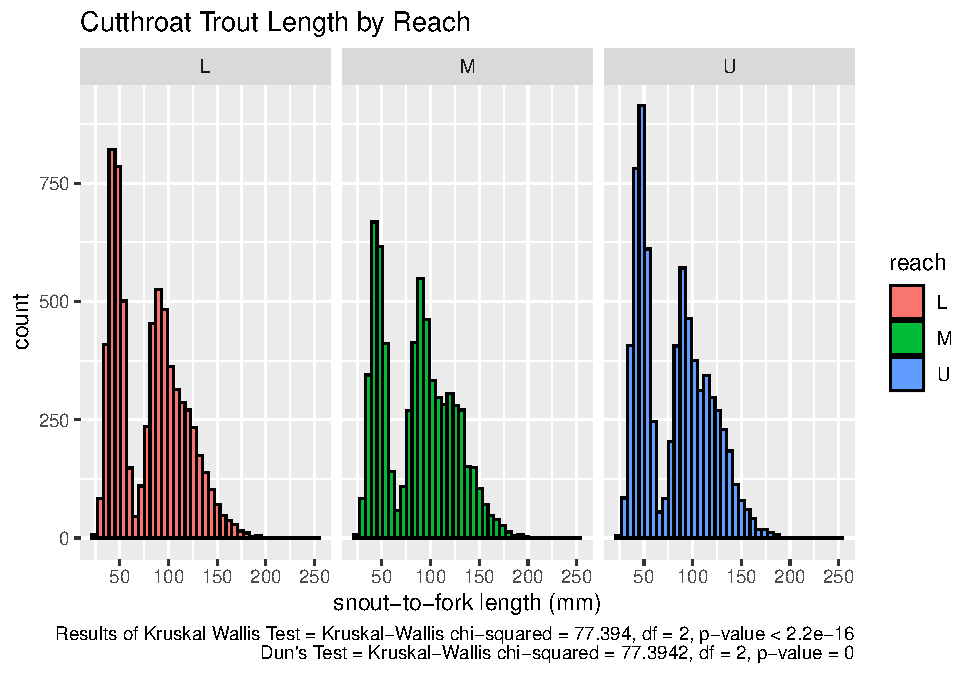
\includegraphics{Lab7_Summer.Heschong_files/figure-latex/vis results-1.pdf}
\#(3) Contingency Tables and the Chi-Squared Test \#\#a. Create a
Contingency Table

\begin{Shaded}
\begin{Highlighting}[]
\CommentTok{\#get data ready for contingency table}
\NormalTok{contingency\_table }\OtherTok{\textless{}{-}}\NormalTok{ trout\_data }\SpecialCharTok{\%\textgreater{}\%}
  \FunctionTok{group\_by}\NormalTok{(reach, unittype) }\SpecialCharTok{\%\textgreater{}\%}
  \FunctionTok{summarise}\NormalTok{(}\AttributeTok{trout\_count =} \FunctionTok{n}\NormalTok{()) }\SpecialCharTok{\%\textgreater{}\%}
  \FunctionTok{pivot\_wider}\NormalTok{(}\AttributeTok{names\_from =}\NormalTok{ unittype, }\AttributeTok{values\_from =}\NormalTok{ trout\_count, }\AttributeTok{values\_fill =} \DecValTok{0}\NormalTok{) }\SpecialCharTok{\%\textgreater{}\%}
  \FunctionTok{column\_to\_rownames}\NormalTok{(}\AttributeTok{var =} \StringTok{"reach"}\NormalTok{)}
\end{Highlighting}
\end{Shaded}

\begin{verbatim}
## `summarise()` has grouped output by 'reach'. You can override using the
## `.groups` argument.
\end{verbatim}

\begin{Shaded}
\begin{Highlighting}[]
\CommentTok{\#create table}
\NormalTok{fish\_counts }\OtherTok{\textless{}{-}}\NormalTok{ contingency\_table }\SpecialCharTok{\%\textgreater{}\%}
  \FunctionTok{gt}\NormalTok{(}\AttributeTok{rowname\_col =} \StringTok{\textquotesingle{}Reach\textquotesingle{}}\NormalTok{) }\SpecialCharTok{\%\textgreater{}\%}
  \FunctionTok{tab\_header}\NormalTok{(}\AttributeTok{title =} \StringTok{\textquotesingle{}Fish Counts by Reach and Habitat Type\textquotesingle{}}\NormalTok{) }\SpecialCharTok{\%\textgreater{}\%}
  \FunctionTok{grand\_summary\_rows}\NormalTok{(}\AttributeTok{columns =} \FunctionTok{c}\NormalTok{(C, I, IP, P, R, S, SC),}
    \AttributeTok{fns =} \FunctionTok{list}\NormalTok{(}\AttributeTok{Total =} \SpecialCharTok{\textasciitilde{}}\FunctionTok{sum}\NormalTok{(., }\AttributeTok{na.rm =} \ConstantTok{TRUE}\NormalTok{)),}
    \AttributeTok{use\_seps =} \ConstantTok{TRUE} 
\NormalTok{    ) }\SpecialCharTok{\%\textgreater{}\%}
    \FunctionTok{data\_color}\NormalTok{(}\AttributeTok{columns =} \FunctionTok{c}\NormalTok{(C, I, IP, P, R, S, SC),}
    \AttributeTok{palette =} \FunctionTok{c}\NormalTok{(}\StringTok{"\#C0D8F0"}\NormalTok{, }\StringTok{"\#5A7ECB"}\NormalTok{), }
    \AttributeTok{alpha =} \FloatTok{0.75}\NormalTok{)}
\NormalTok{fish\_counts}
\end{Highlighting}
\end{Shaded}

\begin{table}[!t]
\caption*{
{\large Fish Counts by Reach and Habitat Type}
} 
\fontsize{12.0pt}{14.4pt}\selectfont
\begin{tabular*}{\linewidth}{@{\extracolsep{\fill}}l|rrrrrrrr}
\toprule
 & C & I & IP & P & R & S & SC & NA \\ 
\midrule\addlinespace[2.5pt]
 & {\cellcolor[HTML]{rgba(129,157,216,0.75)}{\textcolor[HTML]{FFFFFF}{3951}}} & {\cellcolor[HTML]{rgba(150,175,224,0.75)}{\textcolor[HTML]{000000}{7}}} & {\cellcolor[HTML]{rgba(90,126,203,0.75)}{\textcolor[HTML]{FFFFFF}{79}}} & {\cellcolor[HTML]{rgba(192,216,240,0.75)}{\textcolor[HTML]{000000}{1218}}} & {\cellcolor[HTML]{rgba(192,216,240,0.75)}{\textcolor[HTML]{000000}{33}}} & {\cellcolor[HTML]{rgba(165,189,230,0.75)}{\textcolor[HTML]{000000}{2}}} & {\cellcolor[HTML]{rgba(90,126,203,0.75)}{\textcolor[HTML]{FFFFFF}{1205}}} & 220 \\ 
 & {\cellcolor[HTML]{rgba(192,216,240,0.75)}{\textcolor[HTML]{000000}{2984}}} & {\cellcolor[HTML]{rgba(192,216,240,0.75)}{\textcolor[HTML]{000000}{0}}} & {\cellcolor[HTML]{rgba(192,216,240,0.75)}{\textcolor[HTML]{000000}{6}}} & {\cellcolor[HTML]{rgba(91,127,203,0.75)}{\textcolor[HTML]{FFFFFF}{2121}}} & {\cellcolor[HTML]{rgba(170,194,231,0.75)}{\textcolor[HTML]{000000}{94}}} & {\cellcolor[HTML]{rgba(192,216,240,0.75)}{\textcolor[HTML]{000000}{0}}} & {\cellcolor[HTML]{rgba(100,133,206,0.75)}{\textcolor[HTML]{FFFFFF}{1106}}} & 210 \\ 
 & {\cellcolor[HTML]{rgba(90,126,203,0.75)}{\textcolor[HTML]{FFFFFF}{4484}}} & {\cellcolor[HTML]{rgba(90,126,203,0.75)}{\textcolor[HTML]{FFFFFF}{16}}} & {\cellcolor[HTML]{rgba(174,198,233,0.75)}{\textcolor[HTML]{000000}{20}}} & {\cellcolor[HTML]{rgba(90,126,203,0.75)}{\textcolor[HTML]{FFFFFF}{2131}}} & {\cellcolor[HTML]{rgba(90,126,203,0.75)}{\textcolor[HTML]{FFFFFF}{293}}} & {\cellcolor[HTML]{rgba(90,126,203,0.75)}{\textcolor[HTML]{FFFFFF}{7}}} & {\cellcolor[HTML]{rgba(192,216,240,0.75)}{\textcolor[HTML]{000000}{66}}} & 180 \\ 
\midrule 
\midrule 
Total & 11419 & 23 & 105 & 5470 & 420 & 9 & 2377 & — \\ 
\bottomrule
\end{tabular*}
\end{table}

\#\#b. Run a Chi-Squared Test H0: There is no significant effect of
reach on fish counts in different habitat types HA: There is a
significant effect of reach on fish counts in different habitat types

\begin{Shaded}
\begin{Highlighting}[]
\CommentTok{\#run a Chi{-}Squared test}
\NormalTok{chi\_test }\OtherTok{\textless{}{-}} \FunctionTok{chisq.test}\NormalTok{(contingency\_table)}
\end{Highlighting}
\end{Shaded}

\begin{verbatim}
## Warning in chisq.test(contingency_table): Chi-squared approximation may be
## incorrect
\end{verbatim}

\begin{Shaded}
\begin{Highlighting}[]
\NormalTok{chi\_test}
\end{Highlighting}
\end{Shaded}

\begin{verbatim}
## 
##  Pearson's Chi-squared test
## 
## data:  contingency_table
## X-squared = 1925.5, df = 14, p-value < 2.2e-16
\end{verbatim}

\begin{Shaded}
\begin{Highlighting}[]
\CommentTok{\#examine observed counts}
\NormalTok{chi\_test}\SpecialCharTok{$}\NormalTok{observed}
\end{Highlighting}
\end{Shaded}

\begin{verbatim}
##      C  I IP    P   R S   SC  NA
## L 3951  7 79 1218  33 2 1205 220
## M 2984  0  6 2121  94 0 1106 210
## U 4484 16 20 2131 293 7   66 180
\end{verbatim}

\begin{Shaded}
\begin{Highlighting}[]
\CommentTok{\#examine expected counts}
\NormalTok{chi\_test}\SpecialCharTok{$}\NormalTok{expected}
\end{Highlighting}
\end{Shaded}

\begin{verbatim}
##          C        I       IP        P        R        S       SC       NA
## L 3752.684 7.558606 34.50668 1797.634 138.0267 2.957715 781.1655 200.4674
## M 3644.267 7.340234 33.50976 1745.699 134.0391 2.872265 758.5972 194.6758
## U 4022.050 8.101160 36.98356 1926.667 147.9342 3.170019 837.2373 214.8568
\end{verbatim}

\begin{Shaded}
\begin{Highlighting}[]
\CommentTok{\#examine residuals}
\NormalTok{chi\_test}\SpecialCharTok{$}\NormalTok{stdres}
\end{Highlighting}
\end{Shaded}

\begin{verbatim}
##           C          I        IP         P          R          S        SC
## L   5.94861 -0.2481133  9.267928 -19.49757 -11.024245 -0.6797898  19.68796
## M -19.95689 -3.2852680 -5.774192  12.72105  -4.234961 -2.0543727  16.26126
## U  13.62594  3.4500229 -3.478810   6.75895  14.973671  2.6733082 -35.22952
##          NA
## L  1.709388
## M  1.351373
## U -2.999733
\end{verbatim}

Answer: There was found to be a significant effect of reach on fish
counts in different habitat types as determined by a chi-squared test
(x\^{}2 = 1,925.5, p \textless{} 2.2e-16). For each reach L,M, and U
habitat C had the highest fish count.

\end{document}
